\subsection{System Implementation}
We have implemented \oursystem both on Android smartphone and laptop. The user application is implemented on HTC NEW ONE X with azimuth sensor and WiFi , as well as the site-survey tool application. The server side of \oursystem is implemented on ASUS A43S laptop installed Win7 with four 2.20GHz Intel Core i7 processors, 8GB of DDR2-memory.

For the software part of client application, the code for feature extractor module is implemented using C++ and OpenCV library for Android, the remaining parts are implemented in JAVA , the client application runs on the Android Operating System. The site-survey tool application also runs on Android platform. The server side is implemented using C++ and JAVA.
%It is supposed that both server and client access to the same local area network so that they can communicate with each other.
\subsection{Case Study \uppercase\expandafter{\romannumeral1}: Office Environment}
\subsubsection{Site Survey in Office Environment}

As we have the floor plan of the experimental office environment with $60m \times 28m$ area, we annotate each shooting point on the floor plan with its relative geographical coordinates. Figure~\ref{office_site} shows the floor plan of the office, the yellow star is the original point of the office coordinate system, the red line marks the survey track and white dots mark the shooting points, the distance between every two adjacent shooting points is $1.6m$. On each shooting point, we will take pair-photos from two directions, if the shooting point is on the horizontal segment of green line we take photos from north and south, on the vertical segment we take photos from east and west.
\begin{figure}[h!]
\centering
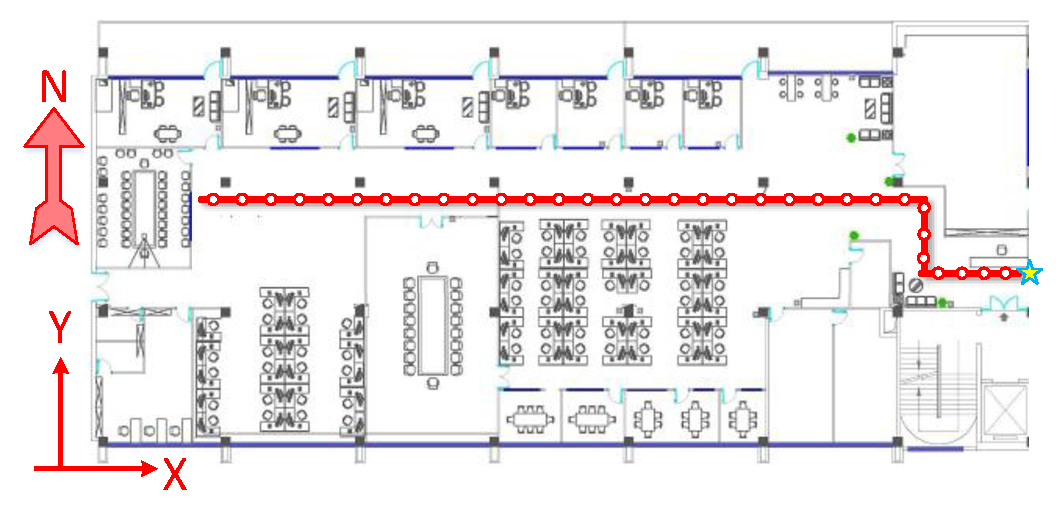
\includegraphics[width=1\linewidth, height=1in, clip,keepaspectratio]{officesite.eps}
\caption{Site survey track in office.}\label{office_site}
\end{figure}

After processing the photos and calculate the geographical locations of reference points, we are able to project the reference points denoted by red points on the floor plan as shown in Figure~\ref{office_ref}. We have filtered out some reference points, the remaining reference points are stable, \ie they are located on the building structure like walls, windows and so on.
\begin{figure}[!htbp]
\centering
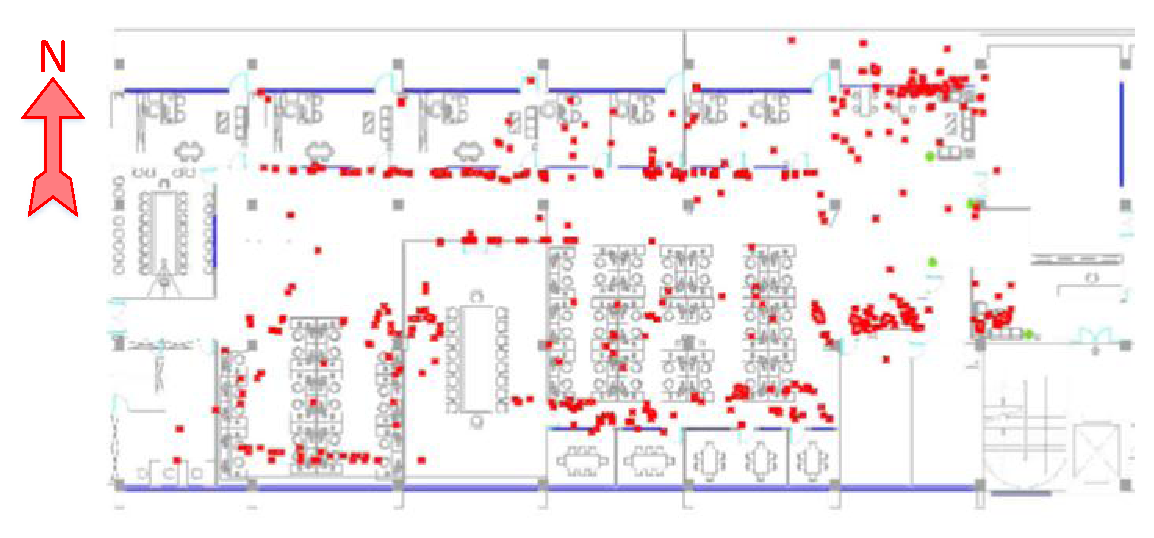
\includegraphics[width=1\linewidth, height=1.1in, clip,keepaspectratio]{officeref4.eps}
\caption{Project filtered reference points on floor plan.}\label{office_ref}
\end{figure}

\subsubsection{Impact of Reference Point Database Size}
In the stage of building up reference point database, the tighter parameters for reference points filtering the less reference points remain, thus we can obtain several reference point databases with different sizes by set different parameters. We study the clustering cost of time and space for a range of sizes of reference point database, Table~\ref{tab_office_cluster} shows the results. As analysed in section~\ref{complexity}, having more reference points results in a longer clustering process, more clusters and larger space, and conversely the less overhead in time and space.
\begin{table}[!htbp]
\centering
\begin{tabular}{ccccc}
\hline
ID &Ref points &Clusters &Time(ms) & \begin{minipage}{2cm}Average cluster size(KB) \end{minipage}\\
\hline
1 &2718 &52 &603 &31.9\\
2 &2088 &46 &371 &27.6\\
3 &1279 &36 &362 &21.75\\
4 &816 &29 &274 &17.3\\
\hline
\end{tabular}
\caption{\label{tab_office_cluster}Impact of reference point database size on clustering stage for office environment.}
\end{table}
\begin{figure*}
\centering
\subfigure[Average LE] {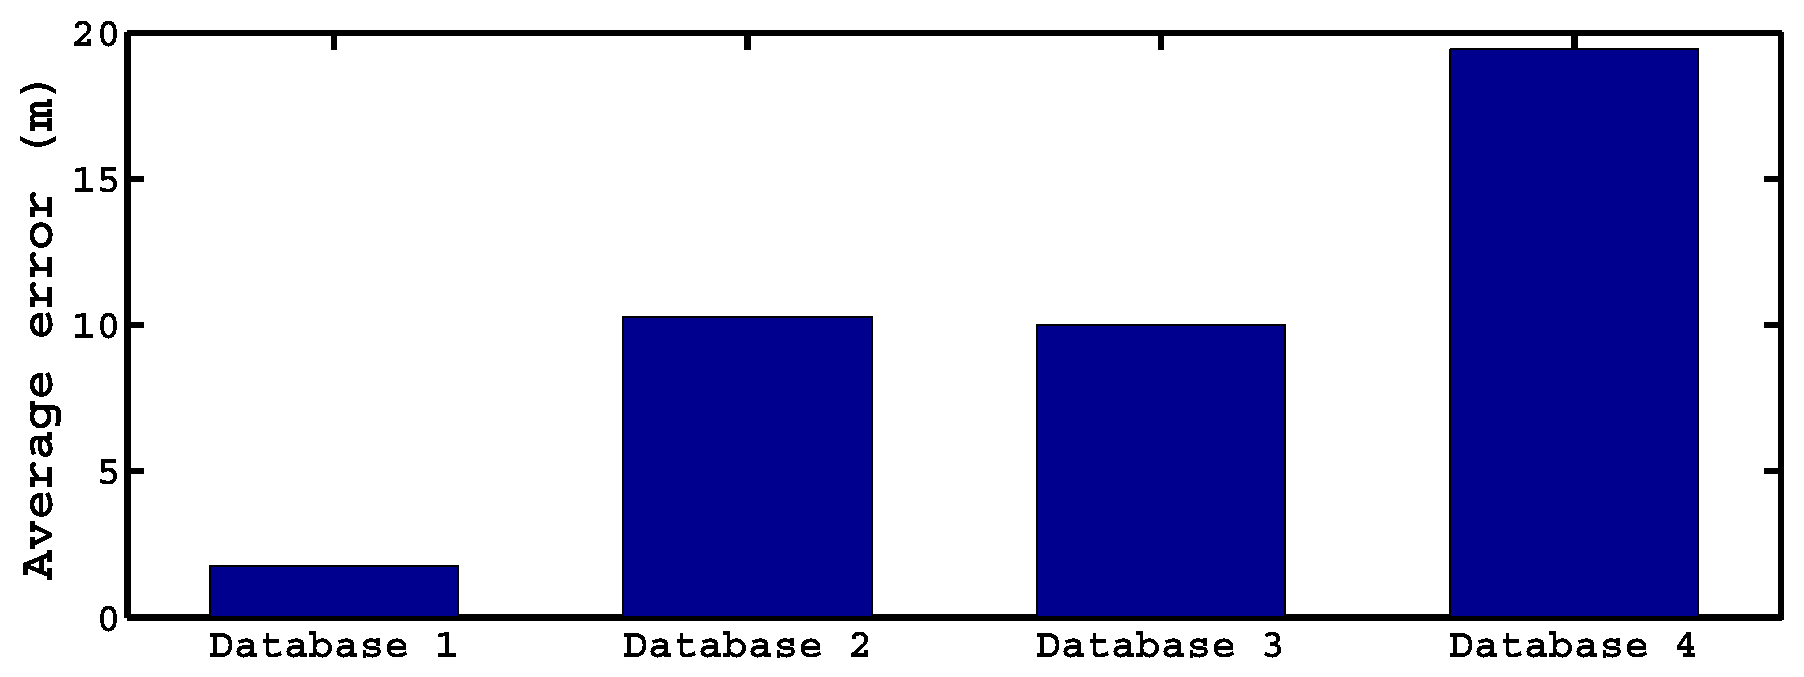
\includegraphics[width=1.7in, height=1.0in]{bar_office4ds.eps}}
\subfigure[CDF of LE] {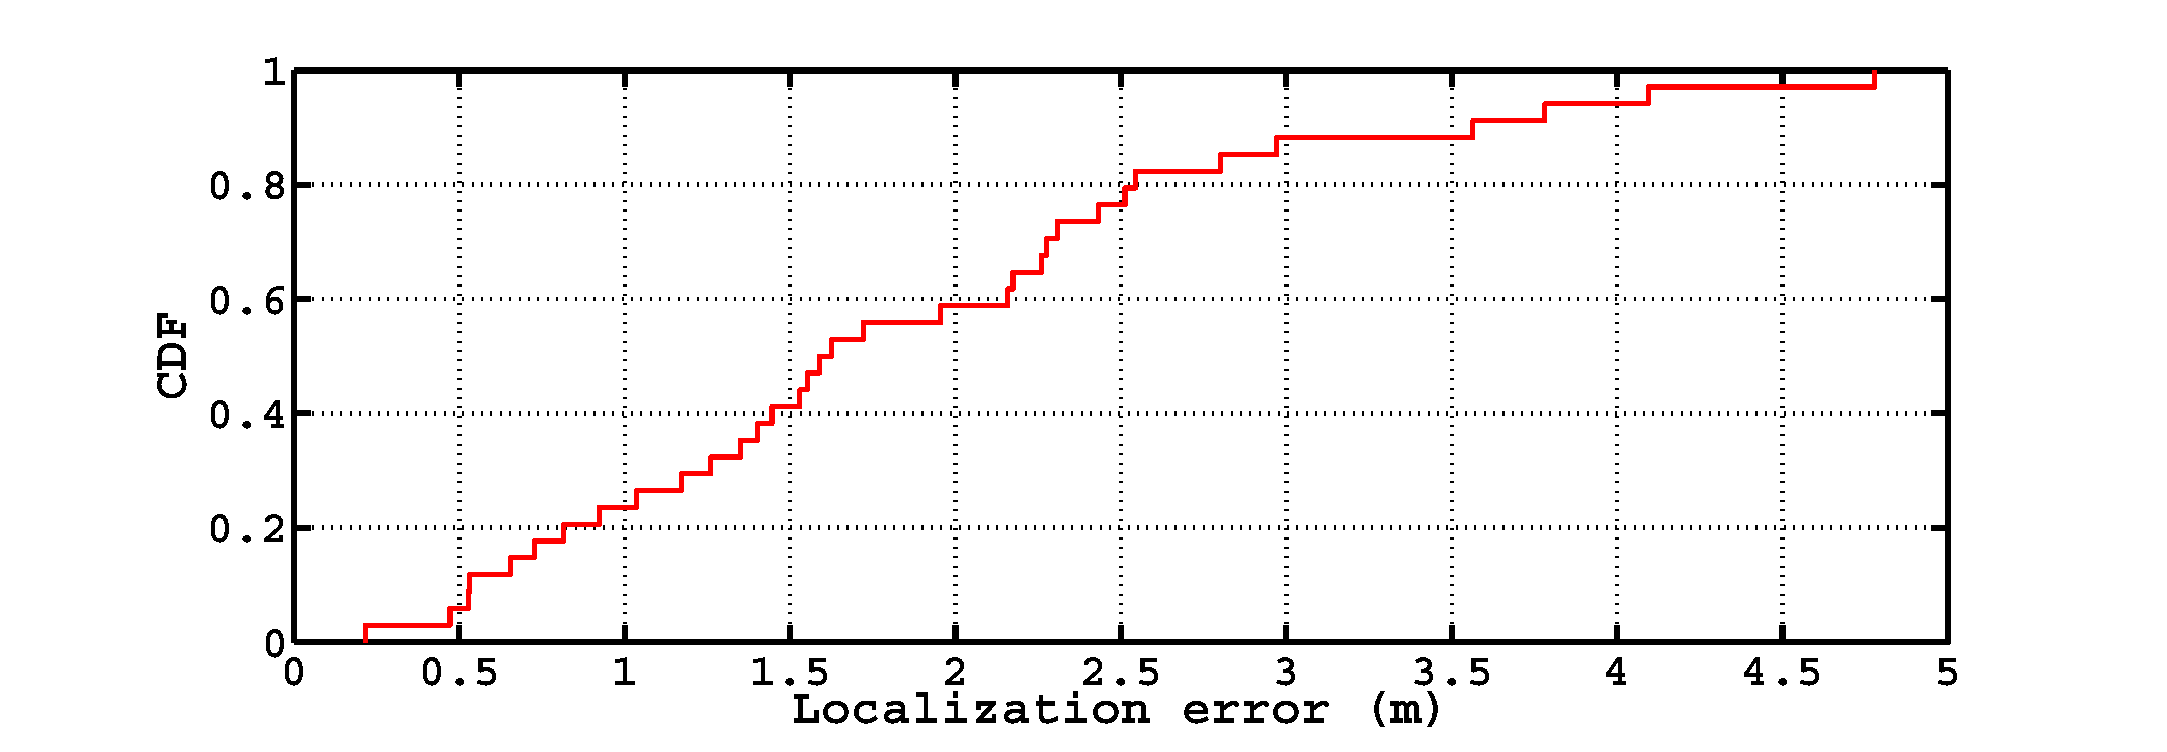
\includegraphics[width=1.7in, height=1.0in]{cdf_Office.eps}}
\subfigure[CDF of LT] {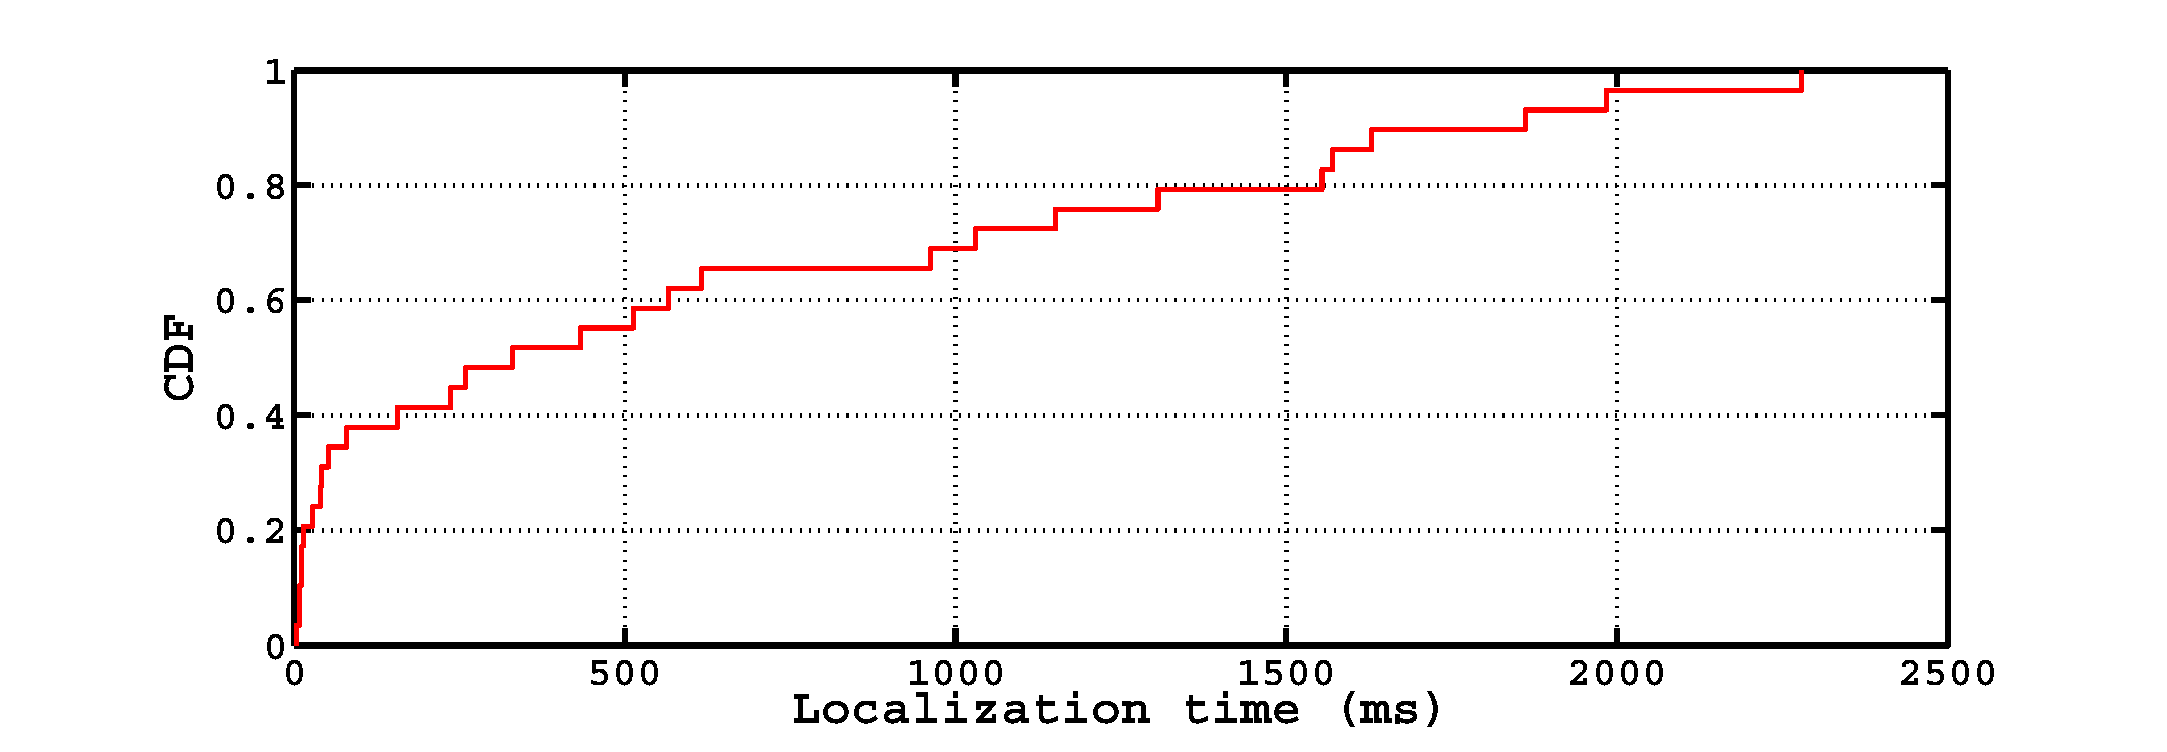
\includegraphics[width=1.7in, height=1.0in]{cdf_office_time.eps}}
\subfigure[CDF of LE] {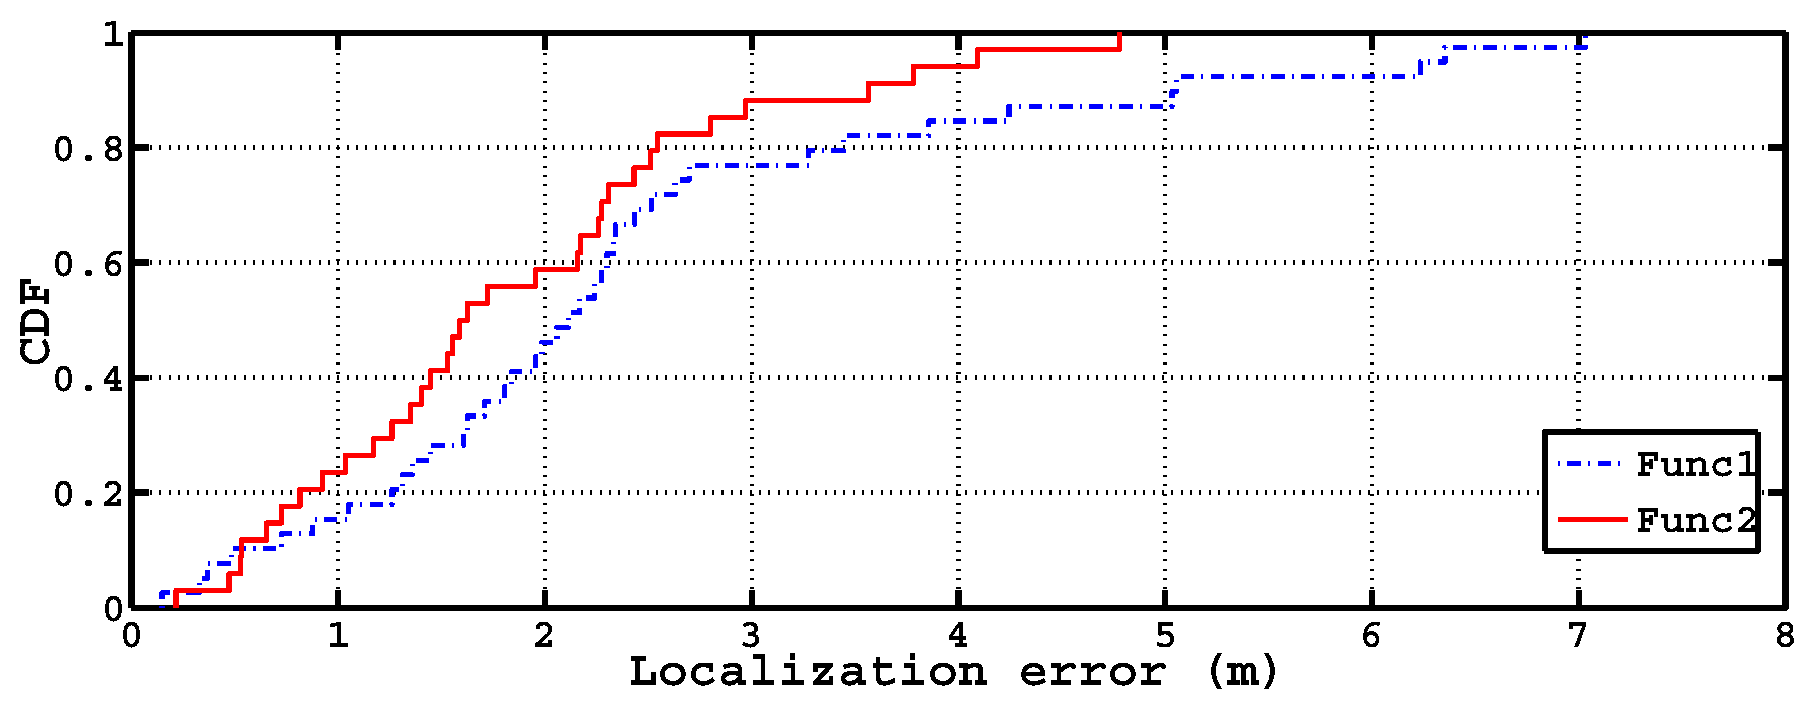
\includegraphics[width=1.7in, height=1.0in]{office_func12.eps}}
\caption{Localization performance in office environment reference database: (a)Average LE of 4 reference point databases. (b)CDF of LE run on database 1. (c)CDF of localization time on database 1.(d)CDF of LE for $Func1$ and $Func2$ in office environment.}
\label{ref_size}
\end{figure*}
Figure~\ref{ref_size}(a) shows the localization error(LE) run on four reference point databases of office environment. Obviously, database 1 which has the largest number of reference points achieves the lowest average error(AE) $1.76m$ among four databases. Database 4 which has the least number of reference points performs a low localization accuracy, its AE is $19.4m$. The AE of database 2 is $10.4m$ which is close to database 3. This result tells us that there is a tradeoff between overhead and localization accuracy, \ie the database with larger size will have more accurate localization results, however, create more overhead and the database with smaller size will cause less overhead but acquire worse localization results. Taking the office environment into account, we are convinced that the size of database for the building whose area is about $1600m^2$ should be almost 2000 reference points.

Figure~\ref{ref_size}(b) shows the CDF of the LE run on database 1. On database 1, we can locate the user with an accuracy of $1.58m$ for 50\% and  $3.56m$ for 91\%. Figure~\ref{ref_size}(c) shows the localization time(LT) run on four office reference point databases, the time of localization process is no more than $2.2s$. With respect to database 1, the localization time is $0.5s$ for 50\% and $1.5s$ for 90\%, which is fast enough to achieve real time localization.

%
%\begin{figure}[t]
%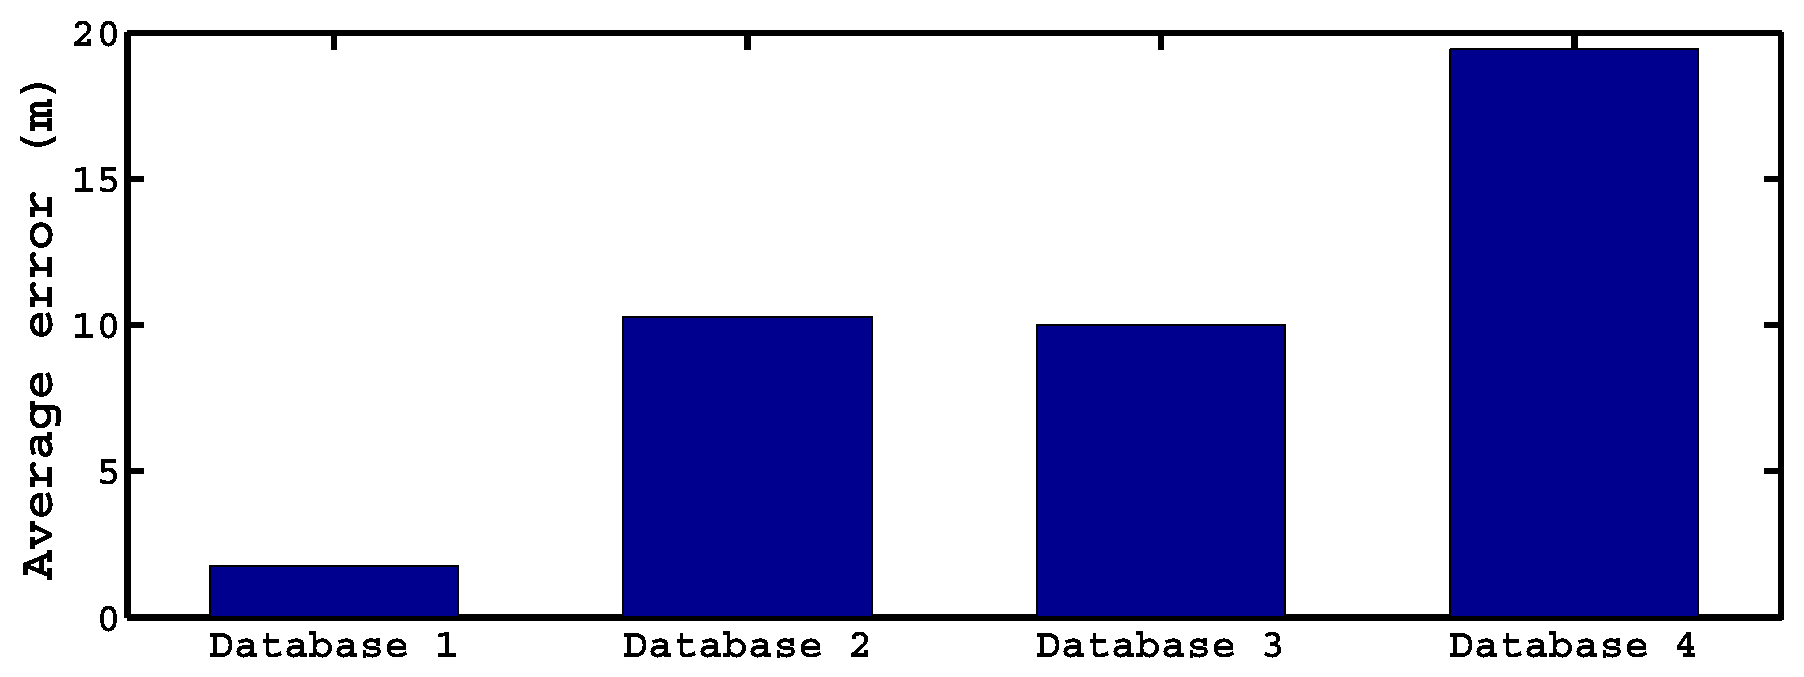
\includegraphics[width=1\linewidth, clip, keepaspectratio]{bar_office4ds.eps}
%\caption{Average LE of 4 reference point databases.}
%\label{bar_office}
%\end{figure}
%\begin{figure}[t!]
%\includegraphics[width=1\linewidth, clip, keepaspectratio]{cdf_office.eps}
%\caption{CDF of LE run on database 1.}
%\label{cdf_office}
%\end{figure}
%\begin{figure}[t!]
%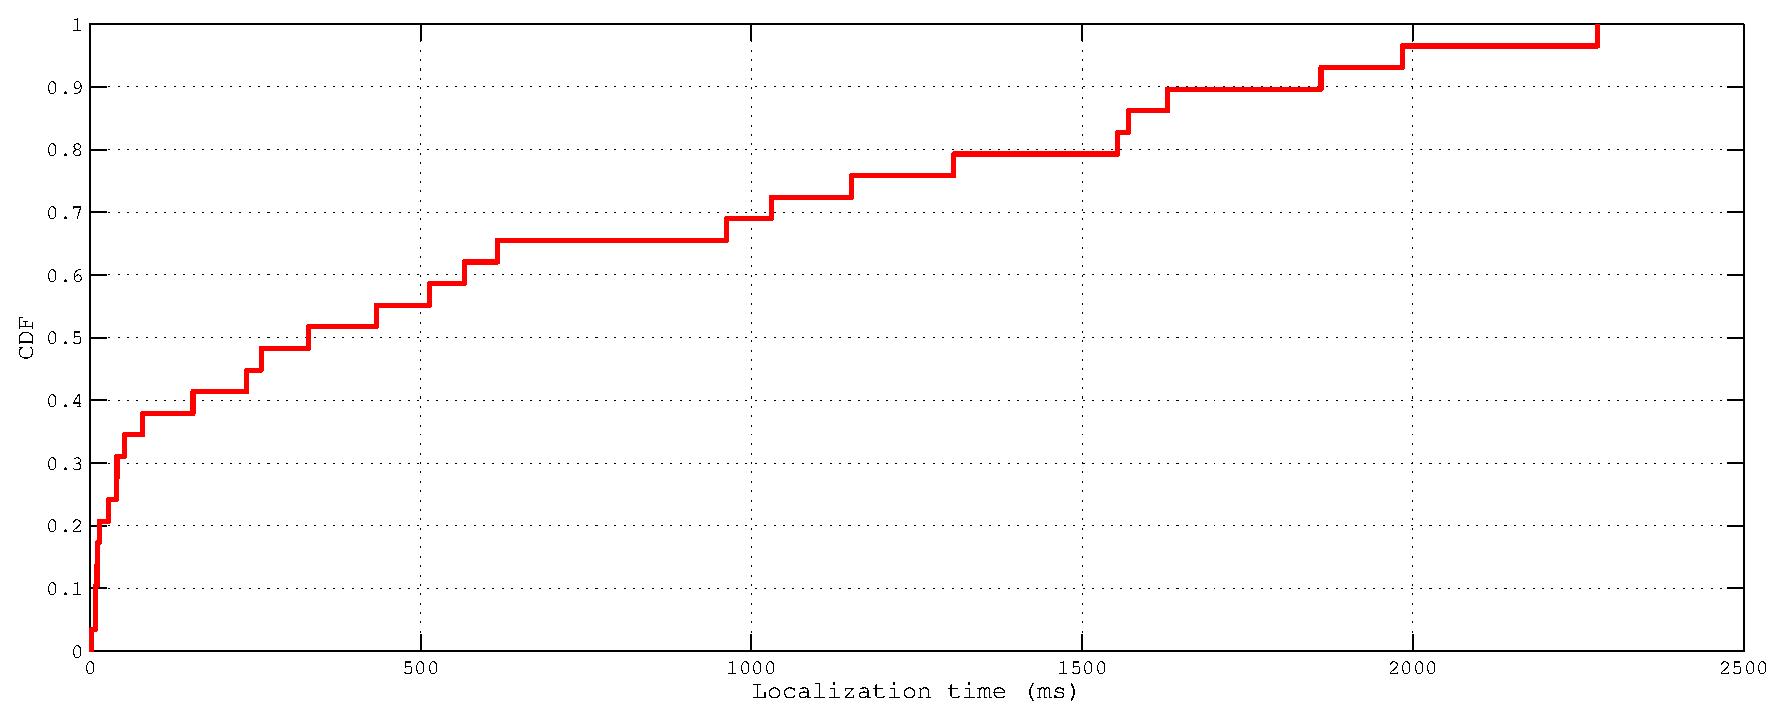
\includegraphics[width=1\linewidth, clip, keepaspectratio]{cdf_officetime.eps}
%\caption{CDF of localization time run on databases 1.}
%\label{cdf_officetime}
%\end{figure}
\subsubsection{Impact of Check Function $Func$}
%This section describes how the size of query point set affects the accuracy of localization. We randomly select $K$ feature point from one query point file to observe the changes of LE. According to the common sense, larger query set should reduce LE. While from Figure~\ref{bar_office_query}, we observe that the LE does not decrease as expected when query set size K increases. The reason for this phenomenon is that more query points may even cause more mismatches between query point and reference point which degenerates the localization accuracy. And LE reaches minimum values when K equals to 25\% or 50\%, which gives us a insight that we can save the communication cost of client by reducing query point set.
%\begin{figure}[t!]
%\centering
%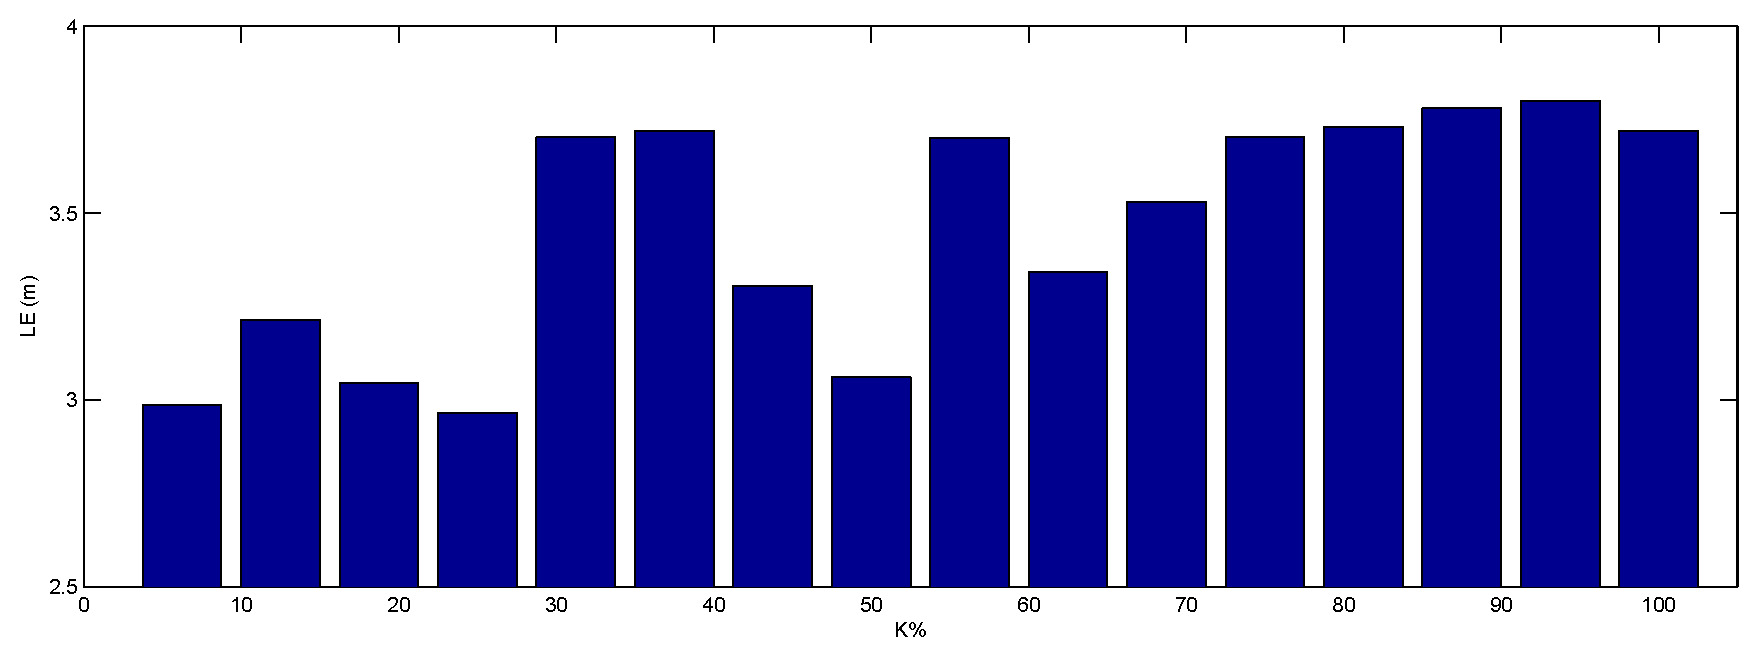
\includegraphics[width=1\linewidth, clip,keepaspectratio]{bar_officequeryK.eps}
%\caption{Average LE of K query feature points.}\label{bar_office_query}
%\end{figure}

%check function%
This section gives an inspection on how different check function $Func$ affect the performance of \oursystem. We use $Func_1$ and $Func_2$ respectively to make accuracy experiments on database 1, the results are shown in Figure~\ref{ref_size}(d). Compared to $Func1$ whose LE is $5.1m$ by 91\%, $Func2$ improves the localization accuracy notably, whose LE is $3.9m$ by 91\%.
%\begin{figure}[!tbp]
%\centering
%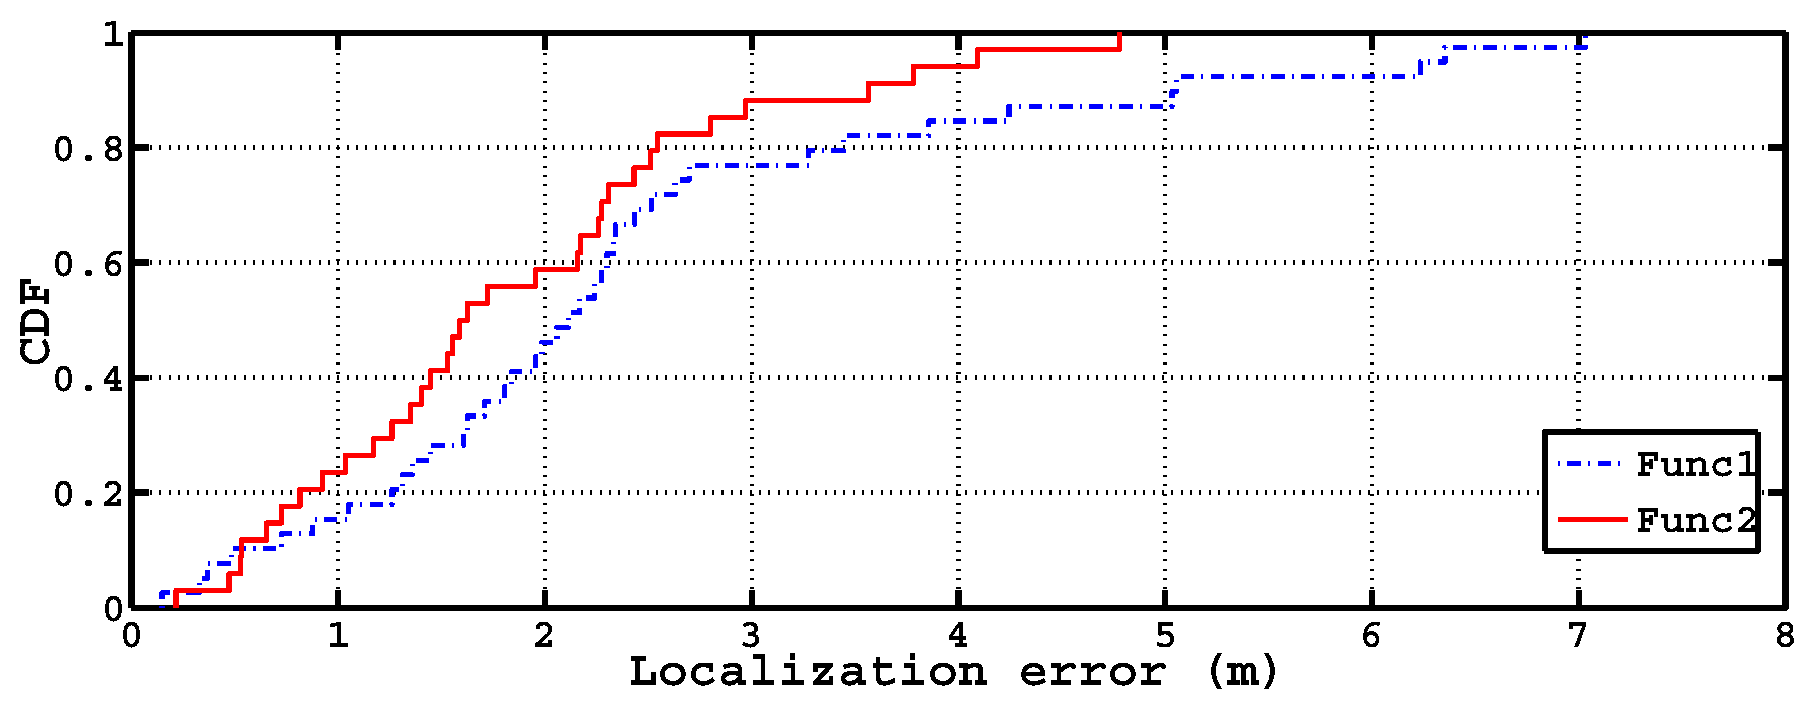
\includegraphics[width=2.2in,height=1.6in, clip,keepaspectratio]{office_func12.eps}
%\caption{CDF of LE for $Func1$ and $Func2$ in office environment.}\label{office_func12}
%\end{figure}
%\subsubsection{Impact of Consensus Estimate Parameters}
%The parameters for consensus estimate also affect the accuracy of \oursystem. Figure~\ref{office_para}(a) shows the AE for different $w$. Figure~\ref{office_para}(b) shows the AE for different $t$.
%\begin{figure}[!htbp]
%\centering
%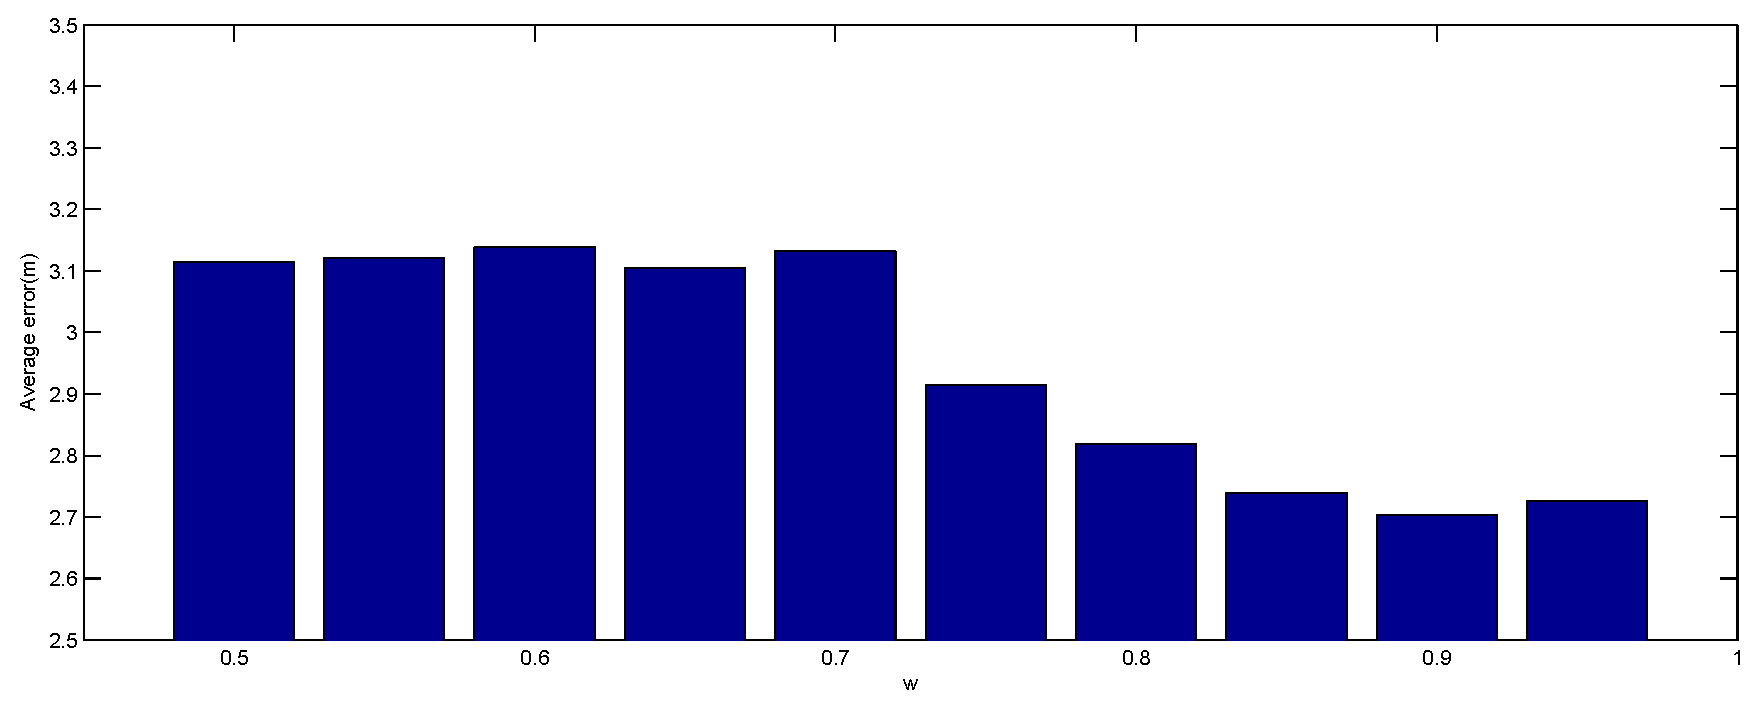
\includegraphics[width=1\linewidth, clip,keepaspectratio]{bar_w_office.eps}
%\caption{Average LE for different $w$.}\label{office_w}
%\end{figure}

%\begin{figure}
%\subfigure[Average error for $w$] {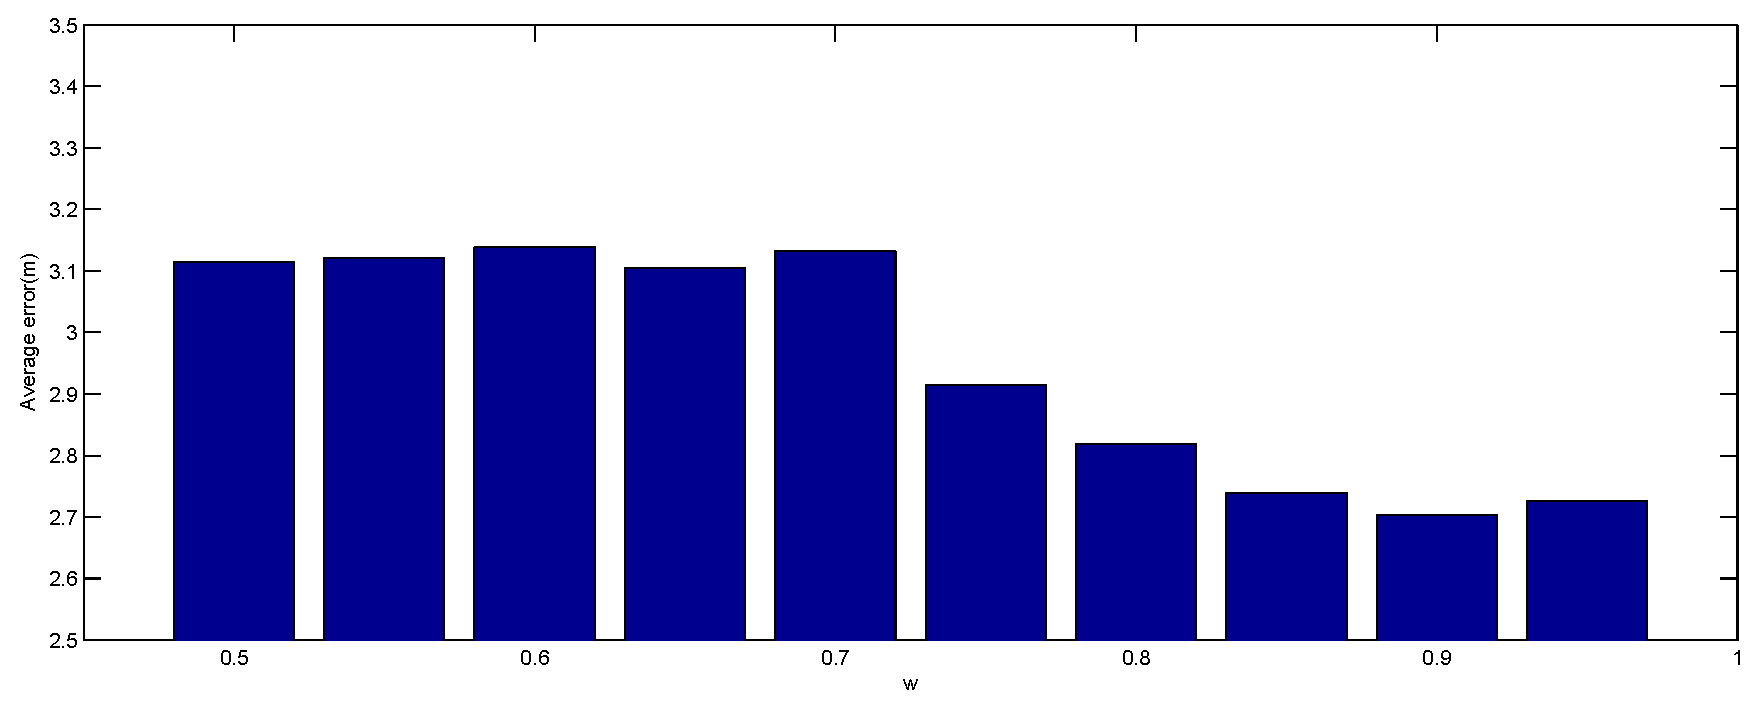
\includegraphics[width=1.4in]{bar_w_office.eps}}
%\subfigure[Avergae error for $t$] {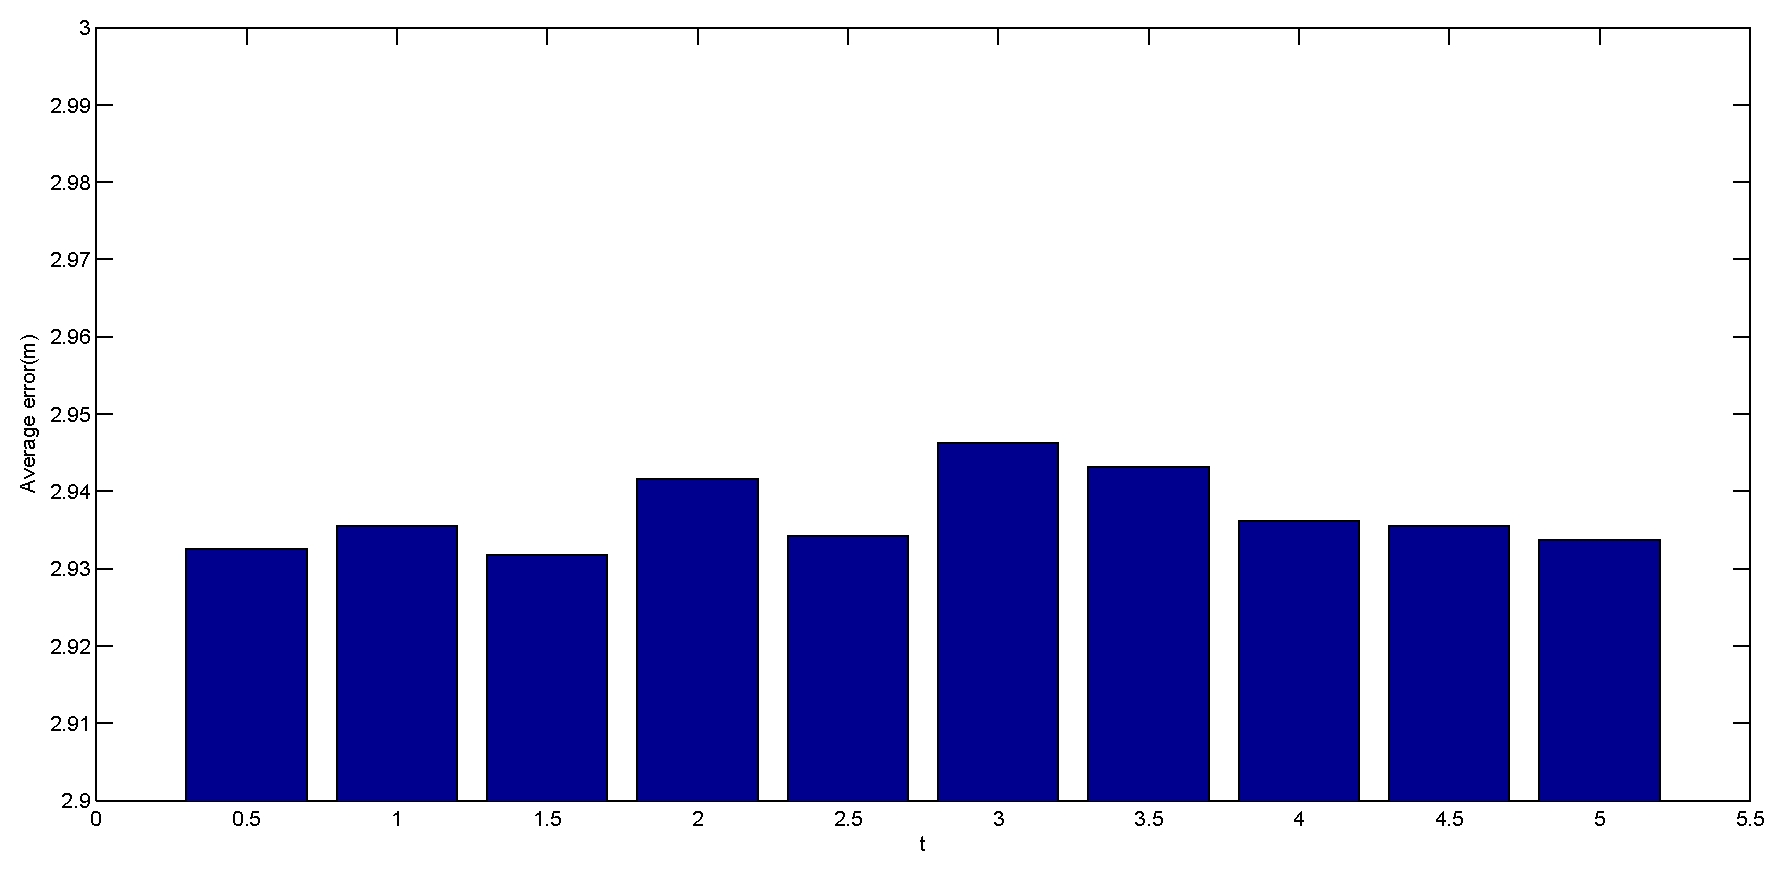
\includegraphics[width=1.4in]{bar_th_office.eps}}
%\caption{Impact of consensus estimate parameters: (a)Average LE for different $w$.(b)Average LE for different $t$.}\label{office_para}
%\end{figure}
\subsection{Case Study \uppercase\expandafter{\romannumeral2}: Shopping Mall}
\subsubsection{Site Survey in Shopping Mall}
We do a site survey for the shopping mall without floor plan, it means that we have to manually mark relative coordinates. Figure~\ref{mall_ref} shows the shooting points by purple diamonds, origin point by red star and filtered reference points by blue crosses. The distance between every adjacent two shooting points is $1.2m$. The shopping mall with $130m\times 13m$ area consists of three little plazas which are connected by two passages. We can tell the shopping mall's structure from the Figure~\ref{mall_ref} which shows the projected reference points.
\begin{figure*}[t!]
\centering
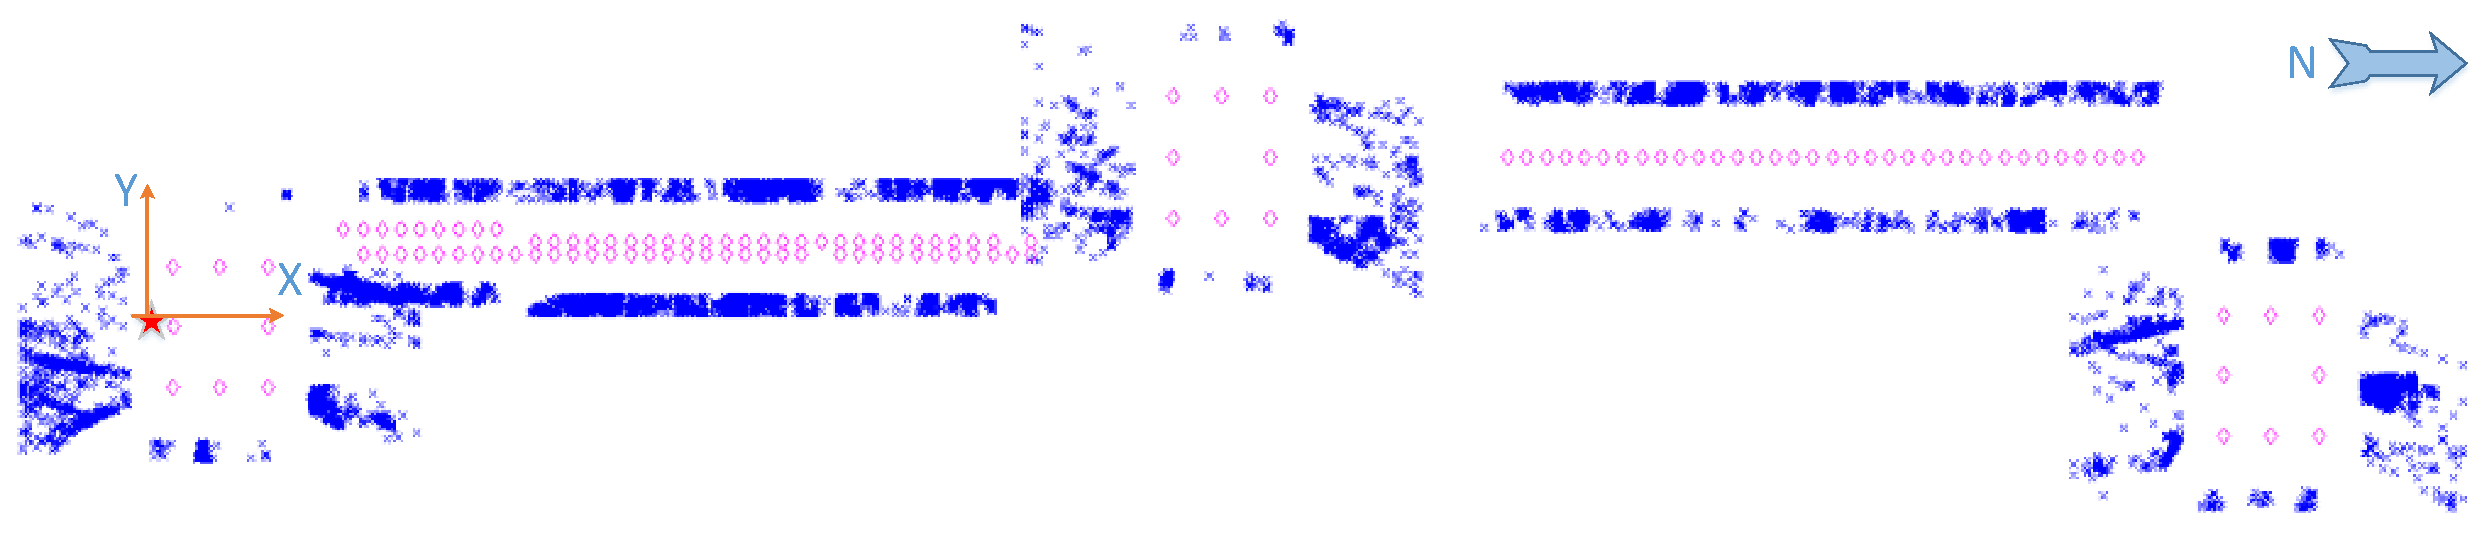
\includegraphics[width=1\linewidth, height=1.1in, clip, keepaspectratio]{mallref2.eps}
\caption{Filtered reference points of shopping mall.}\label{mall_ref}
\end{figure*}
\subsubsection{Reproduction of Results in Previous Work}
In this section, we study the performance of \oursystem in the scenario of shopping mall.
\begin{table}[!htbp]
\centering
\begin{tabular}{ccccc}
\hline
ID &Ref points &Clusters &Time(ms) & \begin{minipage}{2cm}Average cluster size(KB) \end{minipage}\\
\hline
1 &2465 &50 &625 &30.92\\
2 &1739 &42 &516 &26.08\\
3 &1327 &36 &453 &23.36\\
\hline
\end{tabular}
\caption{\label{tab_mall_cluster}Impact of reference point database size on clustering stage for shopping mall.}
\end{table}
Table~\ref{tab_mall_cluster} shows the clustering cost of time and space for a range of size of reference point database in the shopping mall where we conduct experiments on three databases with different sizes.


Figure~\ref{mall_ref_size} shows the localization performance in shopping mall reference point database, which is similar to the results in office environment. As shown in Figure~\ref{mall_ref_size}(a) the AE for database 1 is $2.2m$. The LE run on database1 is $3.4m$ for 90\%, the LT is $1s$ for 90\% as shown in Figure~\ref{mall_ref_size}(b)(c). $Func2$ improves the localization accuracy by $0.7m$ for 90\% queries in shopping mall shown in Figure~\ref{mall_ref_size}(d).
\begin{figure*}
\centering
\subfigure[Average LE]{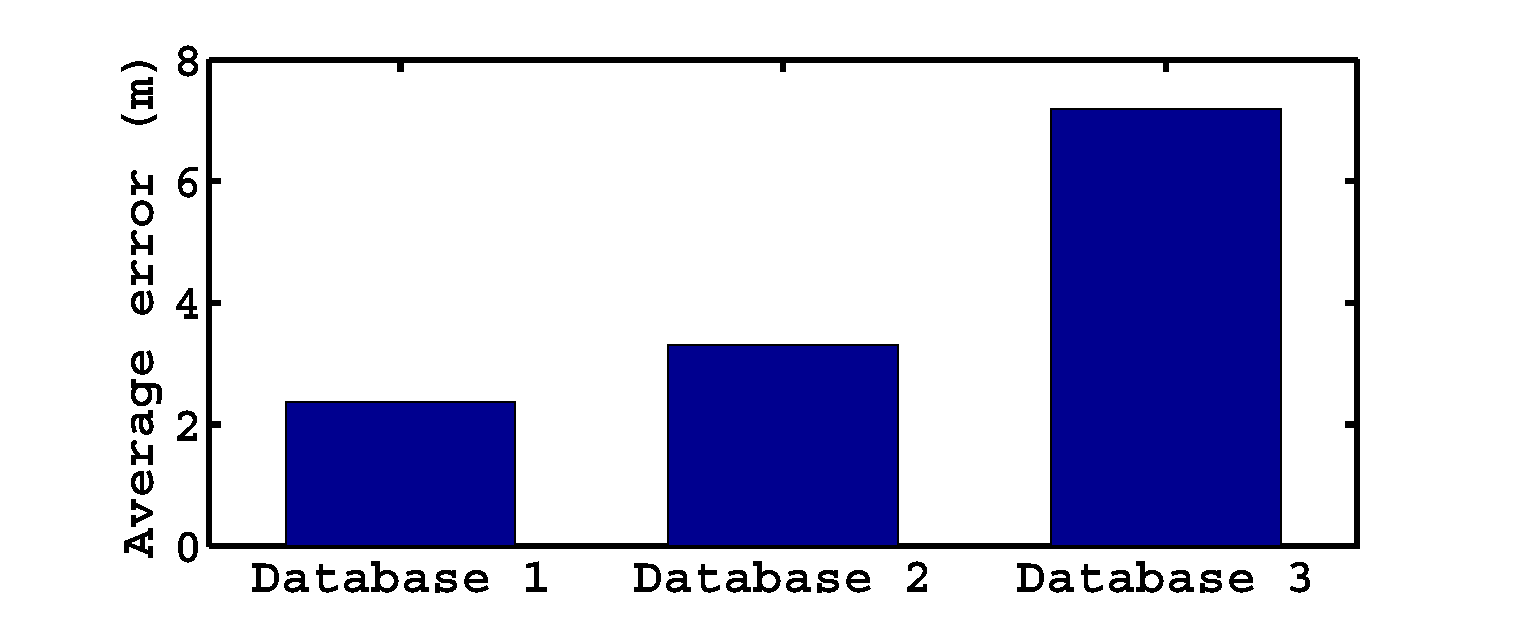
\includegraphics[width=1.7in, height=1.0in]{bar_mall4ds2.eps}}
\subfigure[CDF of LE]{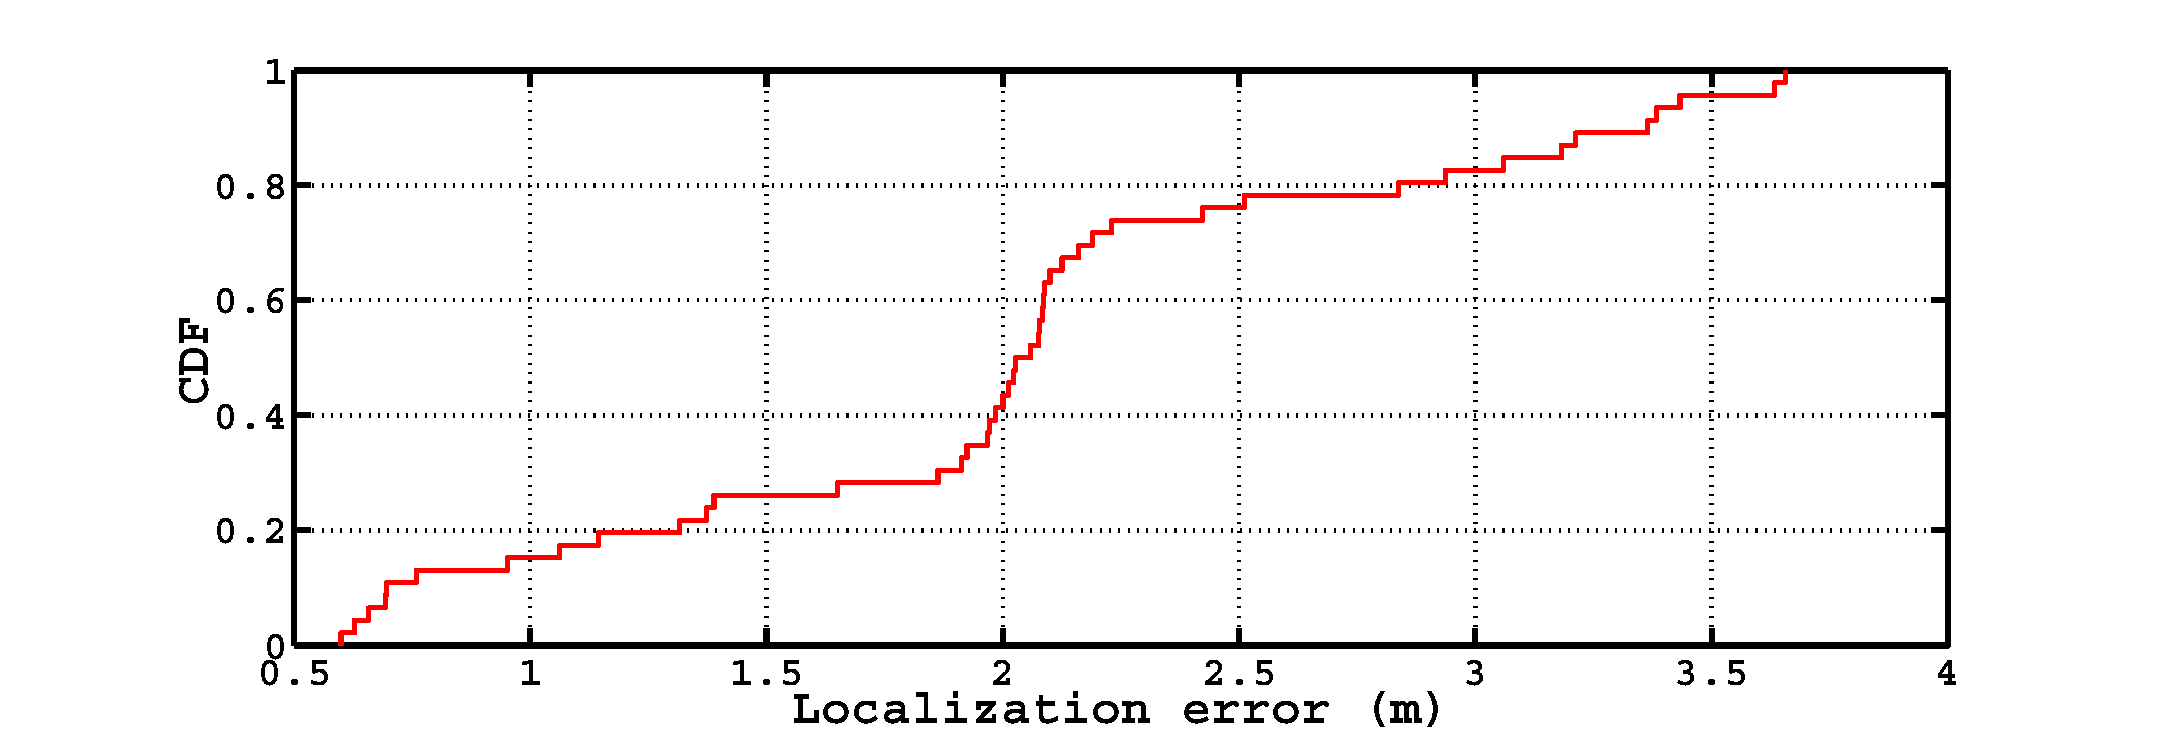
\includegraphics[width=1.7in, height=1.0in]{cdf_mall2.eps}}
\subfigure[CDF of LT]{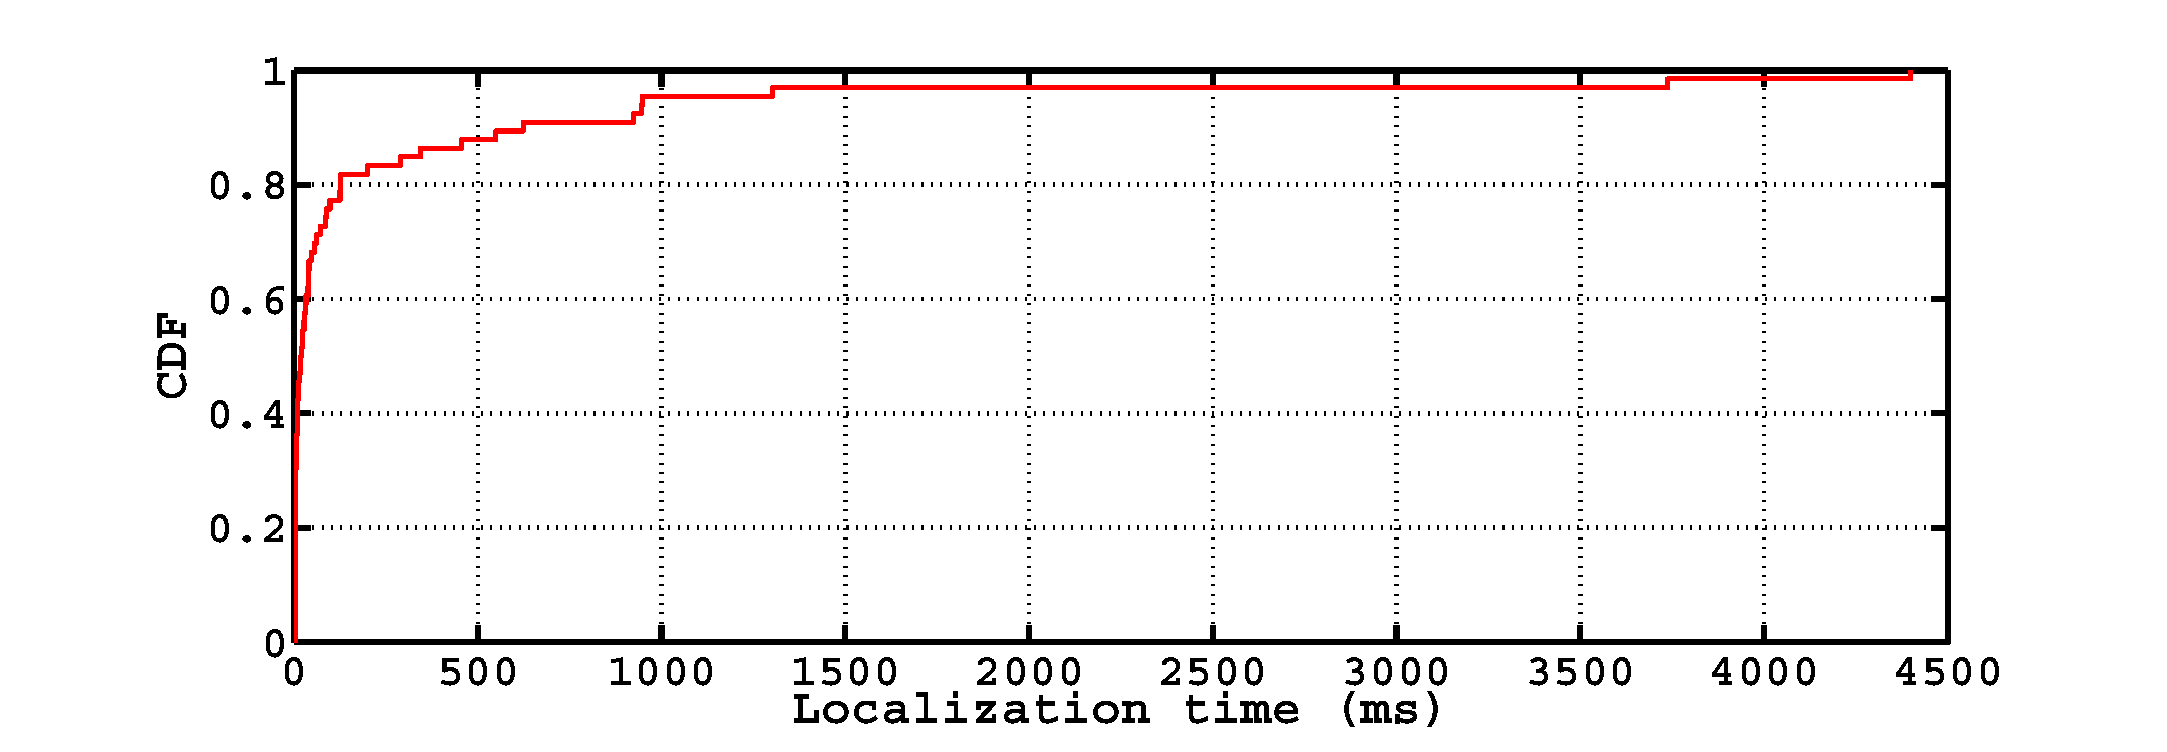
\includegraphics[width=1.7in, height=1.0in]{cdf_malltime2.eps}}
\subfigure[CDF of LE]{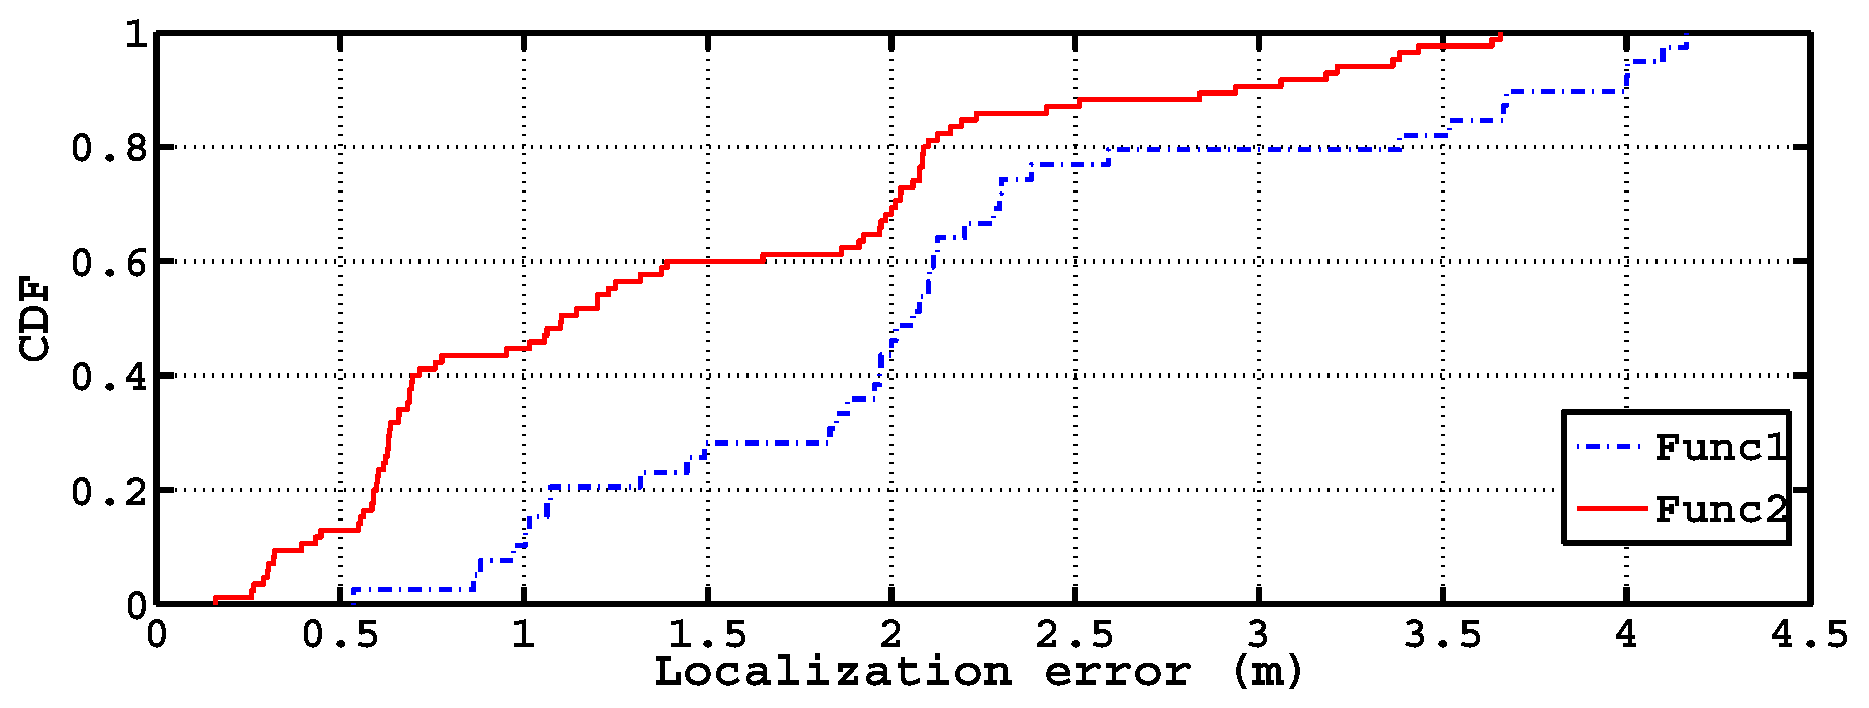
\includegraphics[width=1.7in, height=1.0in]{mall_func12.eps}}
\caption{Localization performance in shopping mall reference points database: (a)Average LE of 3 reference point databases. (b)CDF of LE on database 1. (c)CDF of localization time on database 1.(d)CDF of LE for $Func1$ and $Func2$ in shopping mall.}\label{mall_ref_size}
\end{figure*}
%\begin{figure}[!tbp]
%\centering
%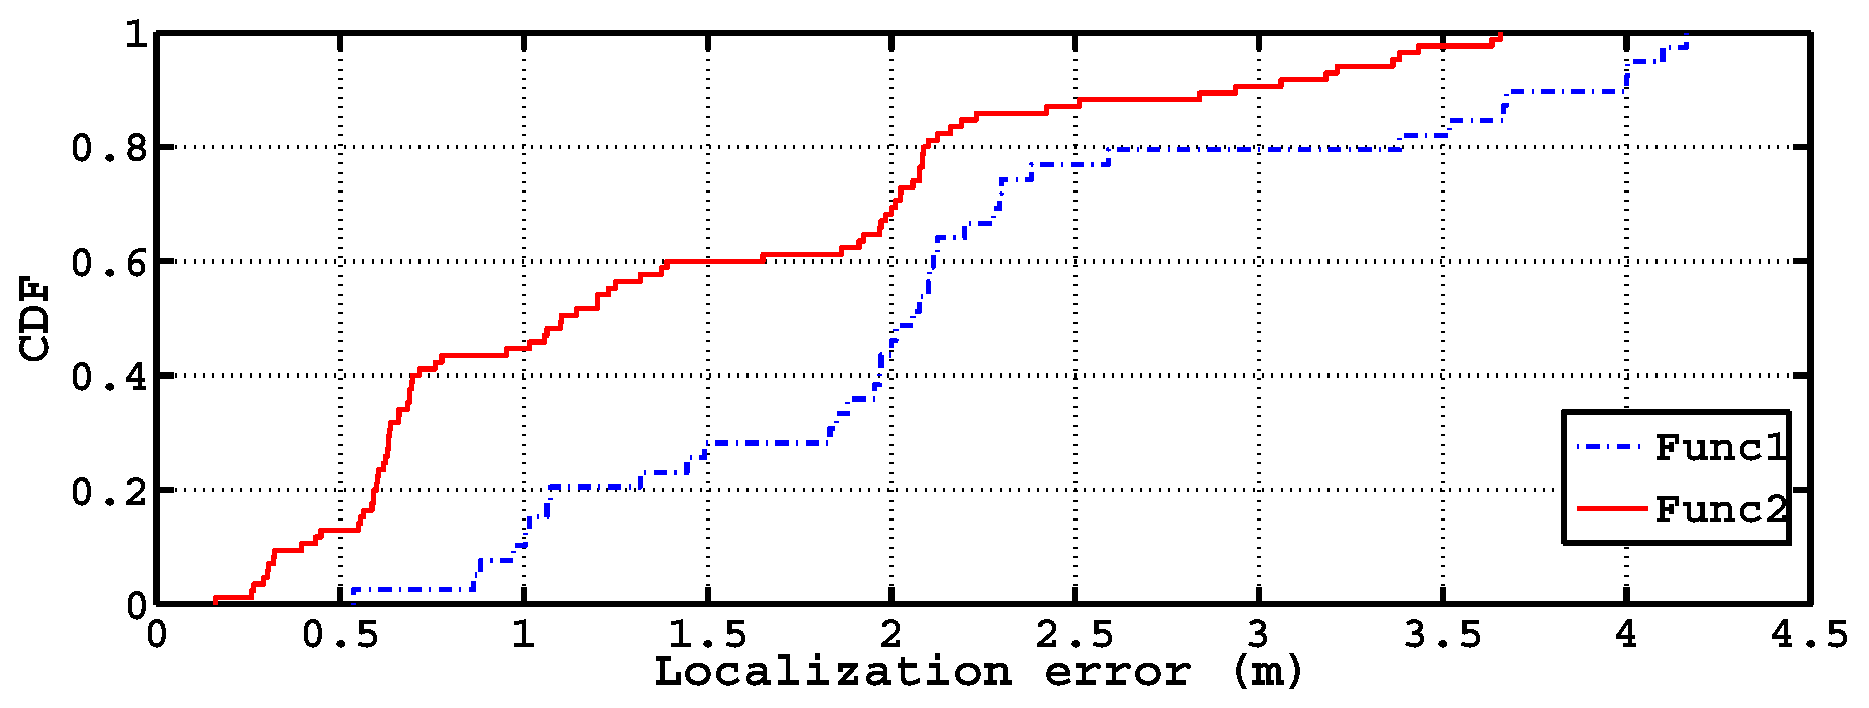
\includegraphics[width=2.2in,height=1.3in, clip,keepaspectratio]{mall_func12.eps}
%\caption{CDF of LE for $Func1$ and $Func2$ in shopping mall.}\label{mall_func12}
%\end{figure}
%\subsection{Communication and Energy Cost}
